\section{Implementación y análisis estadístico de \emph{TRNG} basado en \emph{RO}s}

\subsection{Resumen}

Este capítulo sobre el uso de los osciladores en anillo (\emph{RO}s) como generadores de números aleatorios (\emph{TRNG}).
Se explica el diseño, hecho para \emph{ALTERA Cyclone} III $^{\copyright}$, usando primitivas de bajo nivel.
Se consideran dos características relevantes de un \emph{PRNG} para validar el diseño: 1) el equiprobabilidad de todos los resultados posibles y 2) la estadística independencia de valores consecutivos En este trabajo, estas propiedades se miden a través de Cuantificadores de teoría de la información.
Un plano de doble entropía se usa para representar las series de tiempo y visualizar fácilmente los resultados obtenidos con diferentes configuraciones.
La calidad también se compara con otros \emph{RNG} disponibles por medio del plano de entropía dual.
Nuestro método constituye una reducción efectiva del análisis completo realizado con la prueba suites como \emph{DIEHARD} o \emph{NIST}.

\subsection{Introducción}
\label{sec:Intro}

El jitter y los ruidos de fase presentes en los osciladores en anillo no son convenientes en varias aplicaciones de \emph{RO}s, por ejemplo en la implementación de \emph{osciladores en el chip} para generar relojes en circuitos de alta velocidad \cite{Hajimiri1999, Mandal2010, Gupta2011}.
Sin embargo, son la fuente de aleatoriedad para un \emph{TRNG} basado en \emph{RO}s \cite{Sunar2007, Wold2009}.
Además, un \emph{RO} se puede implementar en un circuito totalmente digital como arreglos de compuertas programables por campo (\emph{FPGA}s) ya que básicamente son solo una serie de inversores.

En \cite{Sunar2007}, Sunar et al. presentó un \emph{PRNG} usando jitter estocástico combinando varios \emph{RO}s.
Ellos requerían un procesamiento posterior del flujo de bits basado en funciones resilientes, para enmascarar imperfecciones en la fuente de entropía y para aumentar inmunidad contra los cambios en las condiciones ambientales.
En ese trabajo se utilizó la entropía del flujo de bits para validar los resultados en.

Wold et al. \cite{Wold2009} propuso una versión mejorada con mejores características aleatorias y sin un procesamiento posterior.
Ellos solo agregaron un flip-flop D adicional en cada salida de anillo.
La efectividad de su propuesta fue probada por medio de suites de prueba disponibles en la literatura abierta \cite{NIST2000, marsaglia1995, NIST2000a}.

En este capítulo se realiza una descripción detallada de una implementación de hardware muy compacta de \emph{TRNG}s basados en \emph{RO}s propuesto en \cite{Wold2009}.
Para validar la aleatoriedad de las secuencias de ruido generadas, se usan dos cuantificadores derivados de la teoría de la información y el plano de doble entropía $H_{BP} \times H_{hist}$ propuestos en la sección \ref{sec:itqs}.
Según lo explicado arriba, $H_{hist}$ es una medida de la equiprobabilidad entre todos los valores posibles y $H_{BP}$ es una medida de la independencia entre valores consecutivos.

A continuación se muestra la implementación de hardware del \emph{RO}s mapeado en \emph{FPGA} Ciclone III y los resultados obtenidos para diferentes configuraciones, comparando estos resultados con los arrojados por otros generadores.

\subsection{Implementación en Hardware}

Los \emph{TRNG} implementados consisten en varios \emph{RO}s con sus salidas XOR juntas y muestreadas por un flip flop \emph{D}.
El flip flop latchea la salida a una frecuencia seleccionada (aquí $ 100 $ MHz) \cite{Wold2009}.
La implementación física se realiza en el kit de desarrollo con \emph{EP3C120F780C7N} \emph{FPGA} cuyo dispositivo principal es una  \emph{ALTERA} $^{\ copyright}$ \emph{Cyclone} III \emph{EP3C120}.
El diseño está hecho con el software \emph{Quartus} $^{\ copyright}$ II 13.1.

\subsubsection{Reseña del Chip}

Las \emph{FPGA}s consisten en una gran cantidad de bloques de matriz lógica (\emph{LAB} s), con grupos de elementos lógicos (\emph{LE} s) para implementar circuitos tanto secuenciales como combinatorios \ref{apendA}.
En la arquitectura de la familia \emph{Cyclone} III cada \emph{LAB} contiene $16$ \emph{LE}s.
Básicamente, cada \emph{LE} es un Flip Flop (\emph{FF}) con una (\emph{LUT}) de cuatro entradas(ver Fig. \ref{fig:LE}).
Cada \emph{LUT} puede implementar cualquier función de vcuatro variables.
El \emph{FF} y el \emph{LUT} se pueden usar juntos o independientemente, \cite{Altera}.

%=========================================
 % FIGURA
\begin{figure}
\begin{center}
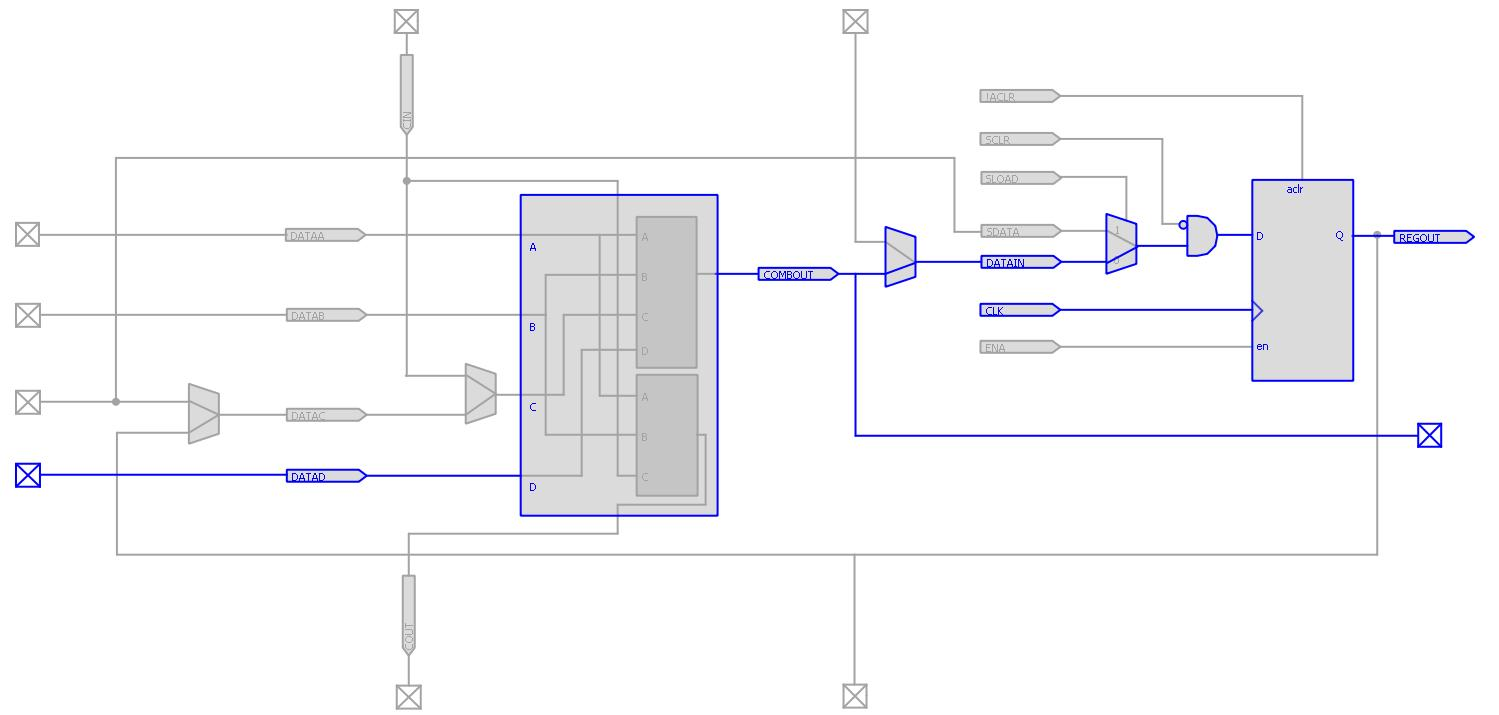
\includegraphics[ width=0.5\textwidth]{NOTenLEmasFF}
\caption{Imagen del Chip Planner que muestra la implementación de un inversor y un Flip Flop.} \label{fig:LE}
\end{center}
\end{figure}
%=========================================

Por lo general, el software de síntesis asigna recursos sin la intervención del diseñador.
Pero en el diseño de \emph{PRNG}s basados en \emph{RO}s es necesario controlar la ubicación exacta de cada componente individual  para evitar la simplificación de los inversores realizada por la herramienta de síntesis.
En \emph{Altera} el uso de primitivas de bajo nivel permite controlar la implementación.
Por consiguiente, estas primitivas y asignaciones de bajo nivel se emplean dentro del código \emph{HDL} empleado en nuestro diseño.
Además, se debe configurar la herramienta de síntesis para evitar que la herramienta de síntesis elimine los búferes redundantes.

Las cadenas de \emph{RO}s se pueden programar en el chip instanciando los \emph{LUT}s como inversores.
Es necesario evitar que el motor de síntesis \emph{Quartus} II fusione dos compuertas \emph{NOT} en serie, utilizando una primitiva llamada \emph{LCELL}.
Una \emph{LCELL} siempre consume una celda lógica y no es eliminada del proyecto durante la síntesis lógica.
Para crear un \emph{RO}, se programan \emph{LCELL}s como búferes de inversor.
Las Figs. \ref{fig:RTL1ring} y \ref{fig:postMap1ring} muestran cómo esta primitiva es implementada por el compilador Quartus II.
%
\begin{figure*}
\begin{center}
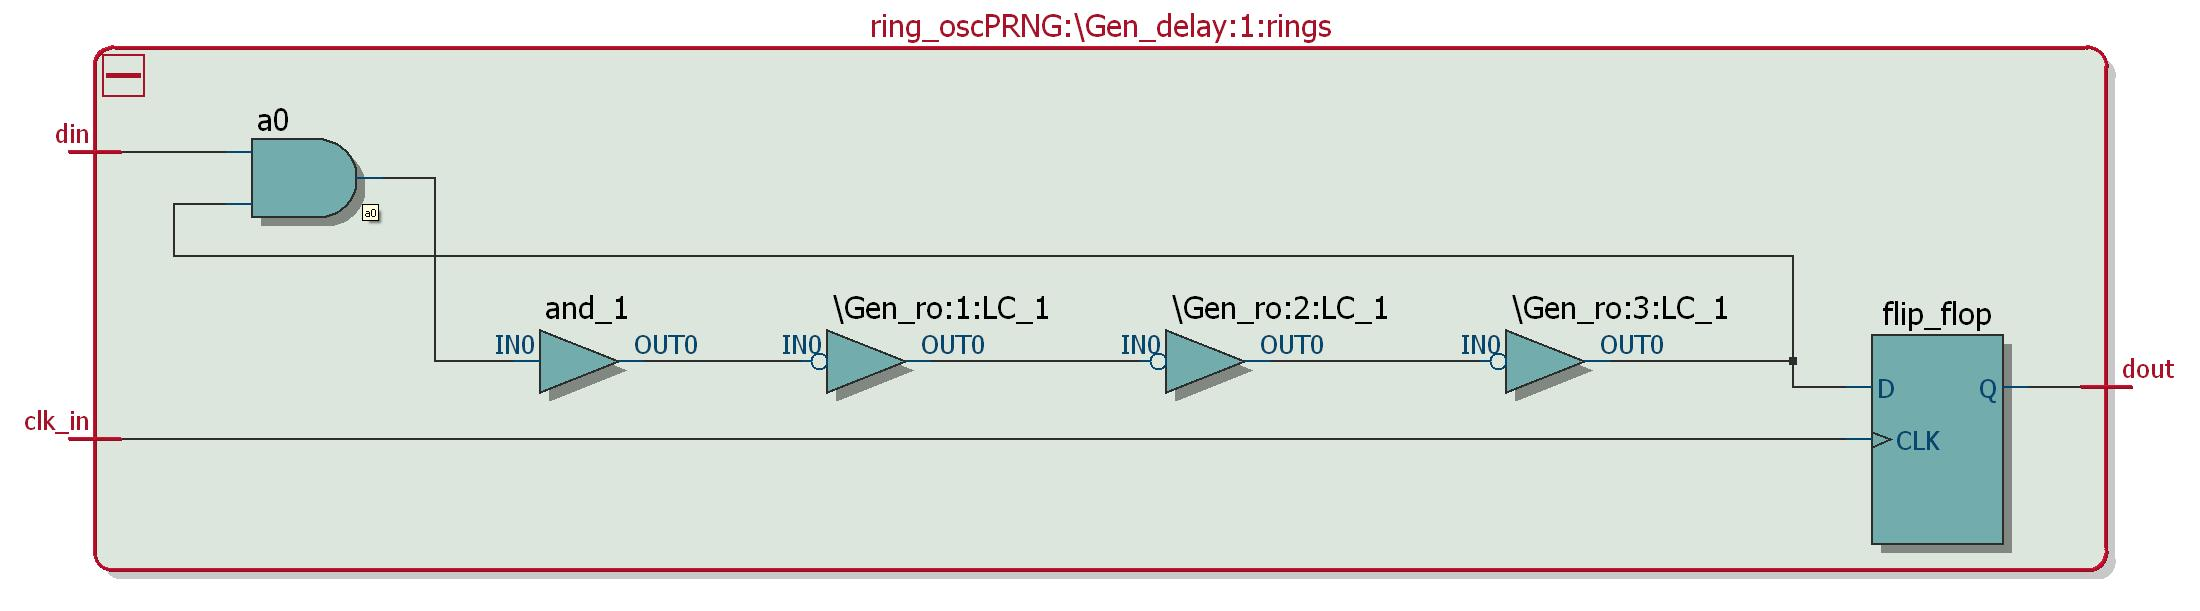
\includegraphics[width=0.7\textwidth]{RTL_view_1ring}
\caption{Vista RTL de un ring con $3$ inversores.}
\label{fig:RTL1ring}
\end{center}
\end{figure*}
%
\begin{figure*}
\begin{center}
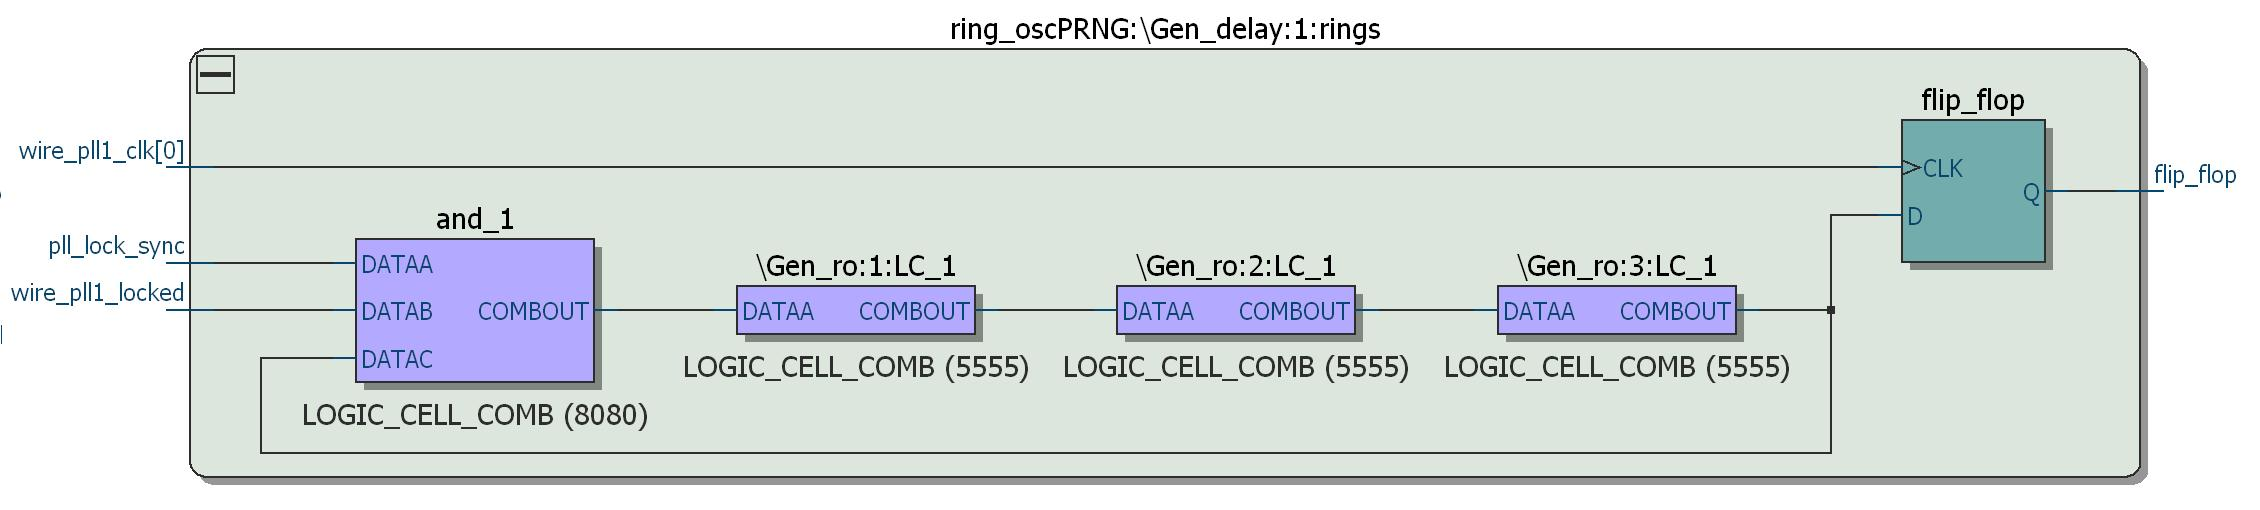
\includegraphics[ width=0.7\textwidth]{tech_map_viewer_post_mapping}
\caption{Technology map viewer (post mapping) de un ring con $3$ inversores.} \label{fig:postMap1ring}
\end{center}
\end{figure*}

Para lograr que cada \emph{RO} tenga comportamientos distintos, cada uno debe ser ubicado en posiciones distintas en el chip.
Para esto debe asignarse a una \emph{LogicLock region} definida previamente.

La Fig. \ref{fig:fpgaplan} muestra las $50$ regiones \emph{LogicLock}s utilizadas para este trabajo.
Se asigna un \emph{RO} a cada región.
Las regiones se distribuyen sobre el chip para un análisis futuro de la importancia de la ubicación.
Cada región tiene $16$ \emph{LAB}s, lo que nos permite aumentar el número de inversores de cada anillo, este es un problema a estudiar en futuros trabajos.

%=========================================
 % FIGURA
\begin{figure*}
\begin{center}
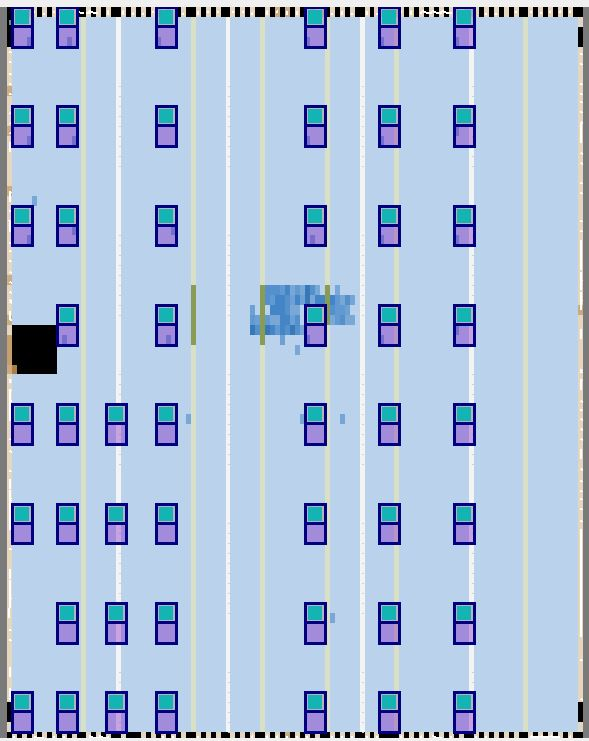
\includegraphics[ width=0.5\textwidth]{fpgaplan}
\caption{Vista de las regiones \emph{LogicLock} del \emph{Chip Planner}.}
\label{fig:fpgaplan}
\end{center}
\end{figure*}

Hay muchos factores que determinan la frecuencia de cada \emph{RO}, y contribuye a la imprevisibilidad de la salida:
\begin{enumerate}

\item Ubicación dentro de \emph{LAB}: las diferentes ubicaciones entre los anillos pueden dar como resultado diferencias de tiempo.
\item Conexiones: incluso teniendo exactamente colocación idéntica de una \emph{LUT} con respecto a la otra en un anillo dado, no es posible tener exactamente el mismo \emph{uso de recursos de enrutamiento} en las conexiones.
\item Selección de entrada: durante la etapa de enrutamiento el \emph{fitter} elegirá qué entrada del \emph{LUT} se utiliza. Como el retraso a través del \emph{LUT} depende de cuál de las cuatro entradas se utiliza, los anillos tienen diferentes retardos.
\item Neighborhood: incluso si todo es bloqueado físicamente, el retardo puede cambiar dependiendo de lo que se coloca y enruta alrededor del anillo.
\end{enumerate}


En la Fig. \ref{fig:RTL3rings} (vista RTL) se muestra un \emph{PRNG} usando $3$ \emph{RO}s seguido por una puerta XOR.
%
\begin{figure}
\begin{center}
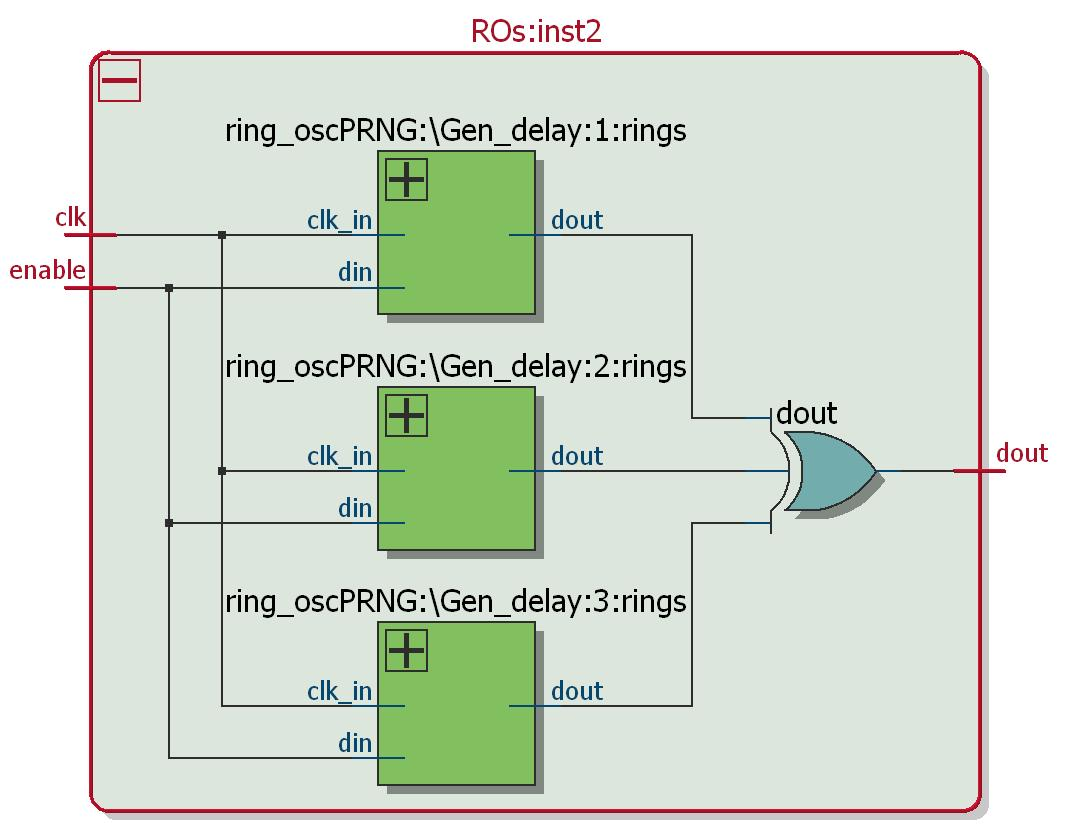
\includegraphics[ width=0.5\textwidth]{RTL_view_3ROs}
\caption{\emph{RTL} de \emph{PRNG} con $3$ \emph{RO}s.}
\label{fig:RTL3rings}
\end{center}
\end{figure}

Para tener una idea de la ocupación en el dispositivo, la tabla \ref{table:compilation} muestra el informe de compilación de un \emph{TRNG} usando $15$ \emph{RO}s cada uno con $3$ inverters.
\begin{table}
\begin{center}
\begin{tabular}{| l | c  c | }
	\hline
	\footnotesize{Total logic elements}          & $847/119,088$       & $( < 1 \%)$  \\ \hline
	\footnotesize{Total combinational functions} & $629/119,088$       & $( < 1 \%)$  \\ \hline
	\footnotesize{Dedicated logic registers}     & $617/119,088$       & $( < 1 \%)$  \\ \hline
	\footnotesize{Total registers}               & $617$               &  \\ \hline
	\footnotesize{Total memory bits}             & $131,072/3,981,312$ & $( 3 \%)$    \\ \hline
\end{tabular}
\end{center}
\caption{Compilation Report, \emph{RO}-based \emph{PRNG} using $15$ \emph{RO}s and $3$ inverters each.}
\label{table:compilation}
\end{table}

\subsection{Resultados}
\label{sec:results}

La herramienta \emph{Embedded Logic Analyzer} se utiliza para recopilar las secuencias aleatorias generadas.
Constituye una \emph{herramienta de depuración a nivel de sistema}, proporcionada por $ Altera $ \cite{CUARTO}, que captura y almacena el comportamiento de la señal en tiempo real y permite observar las interacciones entre el hardware y el software en los diseños del sistema.
Después de adquirir los datos y guardarlos en un archivo \emph{SignalTap} II, pueden ser analizado o visto como una forma de onda.
Con este procedimiento ni jitter adicional, ni la distorsión se introducen en la señal medida de la cadena de adquisición de datos.

Se utilizaron archivos de datos con $917504$ bits cada uno para cada \emph{TRNG}.
Consideramos conjuntos de $N_ {RO}$ anillos, cada uno con $3$ inversores; $N_{RO}=2$, $3$, $4$, $5$, $6$, $7$, $15$, $25$ y $50$.

Data from $SignalTap$ were  processed using \emph{Matlab}$^\copyright$. Binary data were grouped in $6$-bits words without
superposition, so files with $152917$ data each were generated. Quantifiers described in section \ref{sec:method} were calculated
for all generated files.

Los datos de $SignalTap$ se procesaron usando \emph{Matlab} $^\copyright$.
Se agruparon los datos en pañabras de $6$ bits sin superposición, por lo que se generaron archivos con $152917$ datos cada uno.
Se calcularon los cuantificadores descritos en la sección \ref{sec: ITQs} para todos los archivos generados

También evaluamos otros generadores de ruidos conocidos para comparar su calidad con la de los \emph{PRNG} basados en \emph{RO}.
Los ruidos analizados son:

\begin{itemize}
  \item Mersenne Twister pseudo-random number generator, \cite{Matsumoto1998}.
  \item Dos algoritmos empleados para generar datos aleatorios por Matlab (método congruente multiplicativo) \cite{Matlab} y Excel \cite{McLeod1985}.
  \item Dos \emph{ruidos físicos}: ruido de decaimiento radiactivo \cite{Walker2001} y ruido atmosférico \cite{Haahr}.
  Los archivos de datos para estos ruidos están disponibles en los online en los sitios referidos.
  \item Dos mapas caóticos $M^1$ y sus versiones iteradas $M^2$ a $M^8$ \cite{DeMicco2008} para el mapa logístico (\emph{LOGISTIC}) y el \emph{three way Bernoulli map} (\emph{TWBM}).
\end{itemize}

Fig. \ref{fig:HBPvsHhis_all} shows the results in the dual entropy plane $H_{BP}$ vs $H_{hist}$ for all these noises.
It can be seen that the \emph{physical noises}, the algorithmic \emph{Mersenne Twister}, and the \emph{PRNG}s used in \emph{Matlab} $^\copyright$(\emph{rand} function) and \emph{Excel}$^\copyright$ (\emph{RAND} function), have the  maximum value for $H_{BP}$, indicating that all the ordering patterns appear almost the same number of times. However these five noises present very different behavior with respect the $H_{hist}$ quantifier. The \emph{radioactive decay} is the worst, with a value of $H_{hist}$ about $0.5$ indicating that this sequence does not exhibit all possible values in the same proportion. In Fig. \ref{fig:HBPvsHhis_all} the numbers next to each marker for the chaotic sequences, indicate the number of iteration. The iterated maps have higher $H_{BP}$ because of their mixing property \cite{DeMicco2008}.

La Fig. \ref{fig:HBPvsHhis_all} muestra los resultados en el plano de doble entropía $H_ {BP} \times H_{hist}$ para todos estos ruidos.

Se puede ver que los ruidos físicos, el algoritmo \emph{Mersenne Twister} y los \emph{PRNG}s utilizados en \emph{Matlab} $^\copyright$ (función \emph{rand}) y en \emph{Excel} $^\copyright$ (\emph{RAND}), tienen el valor máximo para $H_{BP}$, lo que indica que todos los patrones de orden aparecen casi el mismo número de veces.
Sin embargo, estos cinco ruidos presentan un comportamiento muy diferente con respecto al cuantificador $H_{hist}$.
El \emph{decaimiento radiactivo} es el peor, con $H_ {hist} \sim 0,5$, que indica que esta secuencia no muestra todos los valores posibles en la misma proporción.
Los números al lado de cada marcador para las secuencias caóticas, indican el número de iteraciones.
Los mapas iterados tienen mayor $H_{BP}$ debido a su propiedad de mezcla \cite{DeMicco2008}.
%
\begin{figure*}
\begin{center}
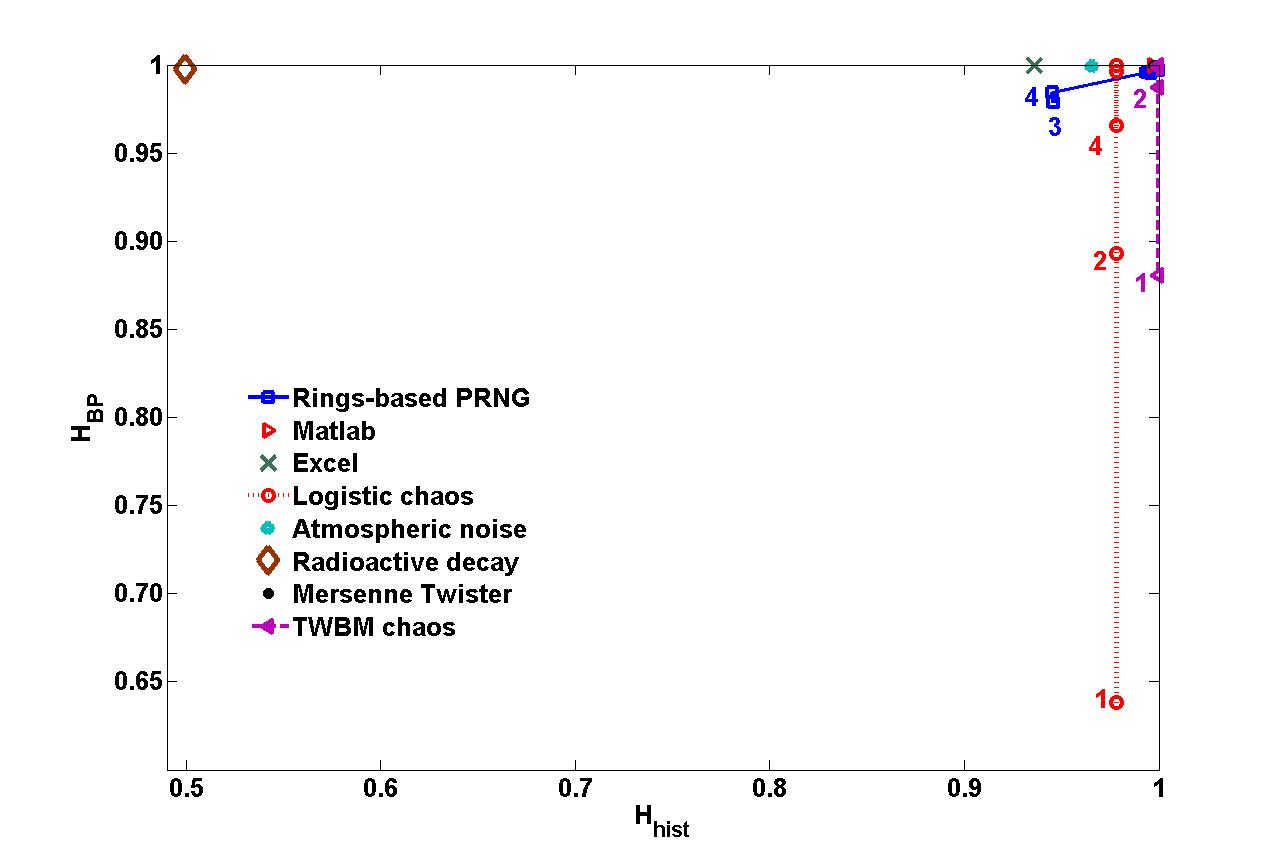
\includegraphics[ width=0.8\textwidth]{HhistvsHBP_t}
\caption{Plano $H_{hist} \times H_{BP}$ para distintos RNGs. Los números que siguen a cada cuadrado indica la cantidad de \emph{RO}s utilizado en cada \emph{TRNG}.
Los números al lado de cada punto en las secuencias caóticas \emph{Logistic} y \emph{TWBM} indican el número de iteración para el mapa caótico (ver texto).}
\label{fig:HBPvsHhis_all}
\end{center}
\end{figure*}

El plano de entropía dual muestra que un aumento en el número de \emph{RO}s mejora tanto $H_ {BP}$ como $H_ {hist}$.

Fig. \ref{HhistvsHBP_zoom} is a zoom of Fig. \ref{fig:HBPvsHhis_all}  around the ideal point $(1,1)$.

La Fig. \ref{HhistvsHBP_zoom} es una vista con más detalle de la Fig. \ref{fig:HBPvsHhis_all} alrededor del punto ideal $(1,1)$.
%
 % FIGURA
\begin{figure*}
\begin{center}
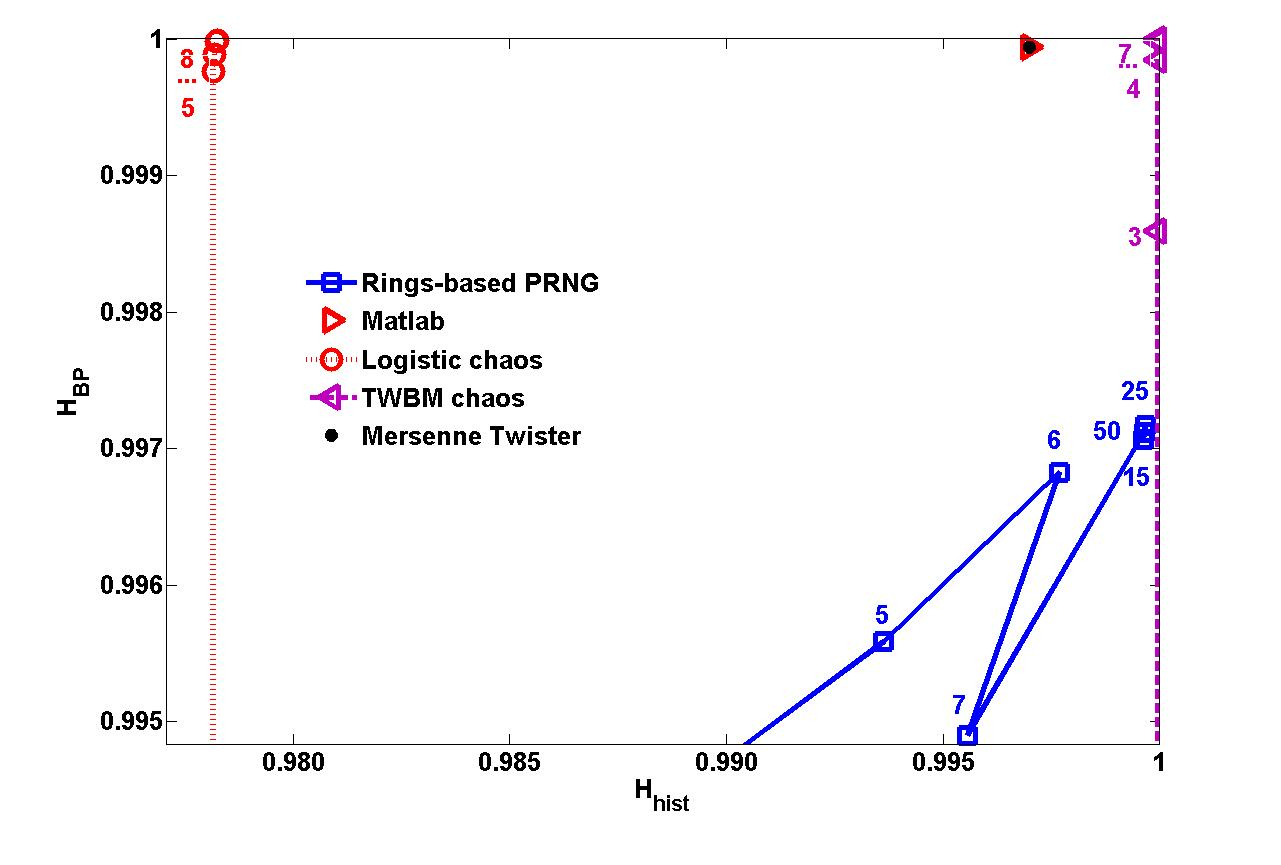
\includegraphics[ width=0.8\textwidth]{HhistvsHBP_z}
\caption{Detalle de la Fig. \ref{fig:HBPvsHhis_all} alrededor del punto ideal $(1,1)$.}
\label{HhistvsHBP_zoom}
\end{center}
\end{figure*}
%
Allí, se muestra la evolución de las secuencias cuando la cantidad de \emph{RO}s aumenta de $5$ a $50$.
Se puede observar que a medida que aumenta el número de anillos los datos aumentan su mezcla y también el histograma tiende a ser más uniforme, por lo tanto, ambas propiedades mejoran.
Se puede determinar un umbral en el número de anillos, ya que los puntos se saturan en alrededor de $(0.997,1)$, por lo que este es el mejor \emph{PRNG} posible, usar más de $15$ \emph{RO}s no presenta ninguna mejora.
Como se dijo anteriormente, el cuantificador $H_ {hist}$ detecta la variación del histograma de la secuencia, y el cuantificador $ H_ {BP} $ refleja la mejora en la mezcla de datos.
Finalmente, las secuencias de Mersenne Twister y Matlab presentan un valor idéntico, ideal $H_ {BP}$ y un valor alto de $H_ {hist}$; no obstante, el histograma no es perfectamente uniforme (los valores no son equiprobables).

\section{Conclusiones}
\label{sec:conclusions}

Los \emph{TRNG}s basados en \emph{RO} implementados aquí han demostrado satisfacer las propiedades estadísticas deseadas para un \emph{RNG}.
Son comparables a otros \emph{RNG}s utilizados y en algunos casos son mejores.
Emplean pocos recursos del dispositivo y se implementan de forma muy simple en una plataforma digital.

It was demonstrated that for these architectures of \emph{PRNG} the quantity of
\emph{RO}s establishes \emph{PRNG}'s statistical properties. It was seen that
for $15$ \emph{RO}s both output's statistical properties, histogram
and mixing, were almost ideal, making unnecessary the increase of the number of rings.

Se demostró que para esta arquitectura la cantidad de \emph{RO}s establece las propiedades estadísticas del \emph{TRNG}.
Se vio que para $15$ \emph{RO}s el histograma y la mezcla, eran casi ideales, haciendo innecesario el aumento de la cantidad de anillos.